\chapter{Acoustics and Digital Signal Processing}
\label{ch:speech analysis}
In the past decade, digital computers have significantly helped \textit{signal processing} to quantify a finite number of bits. The flexibility inherited from digital elements allowed the usage of a vast number of techniques in which had been not possible to implement in the past. Nowadays, digital signal processor have been used to perform multiple operations, such as \textit{filtering}, \textit{spectrum estimation} and many others algorithms \cite{orfanidis1995introduction}.


\section{Speech signals}
\label{sec:speech_signals}
The \textbf{speech} is the human way of communication. The protocol used in communication is based on a syntactic combination of different words taken from a very large vocabulary. Each word in the vocabulary is composed by a small set of vowels and consonants that combined with a phonetic units form a spoken word. \\
\noindent When a word is pronounced\footnote{\ref{ch:english_language} explains in details how phonemes are pronunced}, a sounds is produced causing the air particles to be excited at a certain vibration rate. The source of our voice is due to the vibration of the vocal cords. The resultant signal is a \textit{non-stationary} but it can be divided in segments since each phoneme has a common acoustic properties. In \ref{fig:ex_sound_wave} is possible to notice how the pronounced words have a different shape as well as when the intensity of the voice is higher/lower during the pronunciation.
 
\begin{figure}[!ht]
	\centering
	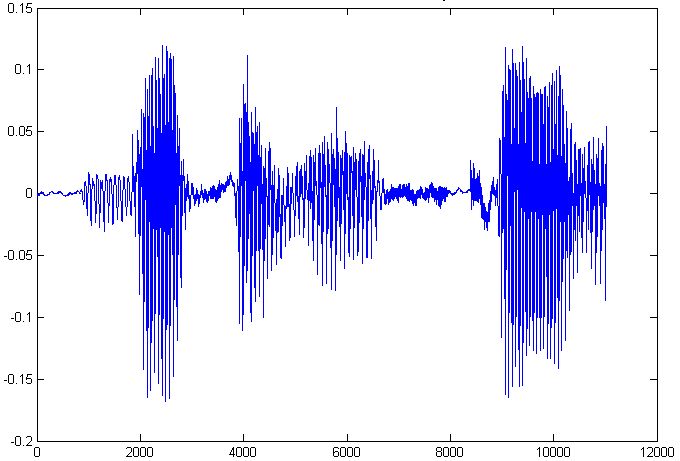
\includegraphics[scale=0.4]{Figures/ex_speech.png}
	\caption{Example of a speech sound. In this case, the sentence "This is a story" has been pronounced \cite{ex_speech_image}}
	\label{fig:ex_sound_wave}
\end{figure}

\noindent The simplest form of sound is the \textit{sinusoid} and it is the easiest waveform to describe because it corresponds to a \textbf{pure tone}. A pure tone consist in a waveform that consists only on one frequency. Other examples are the \textit{cosine} or \textit{sine} waves.

\subsection{Properties of Sinusoids}
\label{sub:prop_of_sinusoids}
A sinusoid, is a simple waveform represented by a up and down movement. There are three important measures that has to be taken into consideration when defining the shape of the sinusoid: \textit{amplitude}, \textit{frequency} and \textit{phase}. 

\subsubsection{Amplitude}
The amplitude, from a sound point of view, corresponds to the \textit{loudness} whereas in the soundwave it corresponds to the amount of \textbf{energy}. In general, to measure the amplitude, we use the unit called \textbf{deciBels} (dB) in which it is measured using a logarithmic scale relative to a standard sound \cite{prop_of_sinusoids}.

\subsubsection{Frequency}
Frequency is the number of cycles per unit of time\footnote{In general, a unit of time is considered a single second}.To define cycle, we can think of an oscillation that starts from the middle line, goes to the maximum point, down to the minimum and get back to the middle point. The unit of measure of the frequency is calculated in \textbf{Hertz} (Hz). Also, if we calculate the time taken for one cycle, we estimate the so called \textbf{period}. \\ 
\noindent Frequency plays a fundamental role with the \textit{pitch}. In fact, changing the number of oscillations but keeping the same waveform, we are able to increase or decrease the level of the pitch.

\subsubsection{Phase}

measures the position of the starting point of the sinusoid. Those starting at the maximum have a phase of zero while those starting at the minimum have a phase of π radians. Phase is best explained with reference to a rotating wheel, see Harrington and Cassidy Chapter 2, Figure 2.7. for more details. The phase of a sinusoid cannot be percieved but we can detect relative changes in phase between two signals, in fact this forms the basis of binaural hearing as the brain works out the location of a sound based on the different phases heard at the two ears.


\subsection{Fourier theory}
\label{sub:fourier_theory}

\subsection{Spectrograms}
\label{sec:spectrograms}



\section{Digital Signals}
\label{sec:digital_signals}



\section{Time Domain Processing}
\label{sub:time_domain_processing}

\subsection{Windowing Signals}
\label{subs:windowing_signals}

\subsection{Time Domain Parameters}
\label{sec:time_domain_params}


\section{Frequency Domain Analysis}
\label{sec:freq_domain_analysis}




\subsection{The Discrete Fourier Transform}
\label{sub:discrete_fourier_transform}

\subsection{Bandwidth}
\label{sub:bandwidth}

\subsection{Frequency Domain Filtering}
\label{sub:frequency_domain_filtering}
